\documentclass[12pt]{article}

%\usepackage{fullpage}
%\usepackage{epic}
%\usepackage{eepic}
%\usepackage{graphicx}

\usepackage{listings} % Code
\usepackage{fancyhdr} % header footer
\usepackage{xcolor}  % Color
\usepackage{mathtools} % Math

\usepackage{geometry}
 \geometry{
 a4paper,
 total={170mm,257mm},
 left=20mm,
 top=20mm,
 }

%\newcommand{\proof}[1]{
%{\noindent {\it Proof.} {#1} \rule{2mm}{2mm} \vskip \belowdisplayskip}
%}


%\newtheorem{lemma}{Lemma}[section]
%\newtheorem{theorem}[lemma]{Theorem}
%\newtheorem{claim}[lemma]{Claim}
%\newtheorem{definition}[lemma]{Definition}
%\newtheorem{corollary}[lemma]{Corollary}

%\setlength{\oddsidemargin}{0in}
%\setlength{\topmargin}{0in}
%\setlength{\textwidth}{6.5in}
%\setlength{\textheight}{8.5in}

\cfoot{footer}

\lstset {
%language=Java,
backgroundcolor = \color{lightgray},
                   language = C++,
                   xleftmargin = 2mm,
                   framexleftmargin = 1em
%lineskip={-1.5pt}
}

%\usepackage[utf8]{inputenc}
 
 
% Information about contents section
%\title{Contents}
%\author{Rudra Nil Basu}
\date{ }
 
%\renewcommand*\contentsname{Summary}

\begin{document}

% to generate the contents page
%\maketitle
\tableofcontents

\newpage

\setlength{\fboxrule}{.5mm}\setlength{\fboxsep}{1.2mm}
\newlength{\boxlength}\setlength{\boxlength}{\textwidth}
\addtolength{\boxlength}{-4mm}
\begin{center}\framebox{\parbox{\boxlength}{\bf
CS593: Programming Practices using C++ \hfill 
Year: 2016
%Date: 11/10/2016
\\
%DATE
\hfill
}}\end{center}
\vspace{5mm}

\section{Pattern}

\textbf{Problem 1.1} \textit{Write a program to print the following pattern using \textbf{for} loop}\\

\begin{lstlisting}
1
22
333
4444
55555
...
\end{lstlisting}

\textit{Code.}

\begin{lstlisting}
#include<stdio.h>
using namespace std;

int main()
{
	int n,i,j;
	scanf("%d",&n);
	for(i=1;i<=n;i++) {
		for(j=1;j<=i;j++) {
			printf("%d",i);
		}
		printf("\n");
	}
}
\end{lstlisting}

\textit{Output.}
\begin{lstlisting}
5
1
22
333
4444
55555
\end{lstlisting}

\section{Average of Cricket Players}

\textbf{Problem 1.2} \textit{A cricket team has the following table of batting figures for a series of test matches
\setlength{\fboxrule}{.5mm}\setlength{\fboxsep}{1.2mm}
%\newlength{\boxlength}\setlength{\boxlength}{\textwidth}
\addtolength{\boxlength}{-4mm}
\begin{center}\framebox{\parbox{\boxlength}{\bf
Player's Name \hfill Runs \hfill Innings \hfill Times not out\\
Sachin \hfill 8430 \hfill 230 \hfill 180\\
Saurav \hfill 4200 \hfill 130 \hfill 9\\
Rahul \hfill 3350 \hfill 105 \hfill 11
}}\end{center}
\vspace{5mm}
% End of box
Write a program to read figures from the above form, to calculate the batting average and print out the complete table including the average
}
%\\


\textit{Code.}

\begin{lstlisting}
#include<stdio.h>
#include<vector>
#include<iostream>
using namespace std;

typedef struct stats {
	char name[50];
	int runs;
	int innings;
	int not_out;
	float average;
}stats;

int main()
{
	int i,n;
	char strtr[10];
	
	int ans;
	while(1) {
		stats players;
		printf("Enter name:");
		scanf("%s",players.name);
		printf("Enter runs, innings, not_out for %s\n",
		players.name);
		scanf("%d %d %d",&players.runs,&players.innings,
		&players.not_out);
		players.average=players.runs*1.0/players.innings;
		g.push_back(players);
		printf("Want more ?(1/0)\nyes=1\tno=0\n");
		scanf("%d",&ans);
		if(ans==0) {
			break;
		}
	}
	printf("Name\tRuns\tInnings\tNot Out\tAverage\n");
	for(i=0;i<g.size();i++) {
		printf("%s\t%d\t%d\t%d\t%f\n",g[i].name,
		g[i].runs,g[i].innings
				,g[i].not_out, g[i].average);
	}
	return 0;
}
\end{lstlisting}

\textit{Output.}
\begin{lstlisting}
Enter name:Rahul
Enter runs, innings, not_out for Rahul
3350 105 11
Want more ?(1/0)
yes=1   no=0
1
Enter name:Sachin
Enter runs, innings, not_out for Sachin
8430
230 18
Want more ?(1/0)
yes=1   no=0
1
Enter name:Saurav
Enter runs, innings, not_out for Saurav
4200 130 9
Want more ?(1/0)
yes=1   no=0
1
Enter name:ThePhenomenalRNB
Enter runs, innings, not_out for ThePhenomenalRNB
8888 105 18
Want more ?(1/0)
yes=1   no=0
0
Name    Runs    Innings Not Out Average
Rahul   3350    105     11      31.904762
Sachin  8430    230     18      36.652172
Saurav  4200    130     9       32.307693
ThePhenomenalRNB        8888    105     18      84.647621
\end{lstlisting}

\section{Electricity}

\textbf{Problem 1.3} \textit{Calculate electric charge for the following rates\\
For first 100 units \hfill 60P per unit\\
For next 200 units \hfill 80P per unit\\
Beyond 300 units \hfill 90P per unit\\
Minimum charge is Rs. 50.00. If total amount is more than 300.00, additional 15\% charge is added.\\
Read names of users and units consumed and print the charge with names
}\\

\begin{lstlisting}
1
22
333
4444
55555
...
\end{lstlisting}

\textit{Code.}

\begin{lstlisting}
#include<stdio.h>
using namespace std;

typedef struct charge {
	char name[50];
	int units;
	float cost;
}charge;

float findCost(int n)
{
	float c=0;
	if(n>=100) {
		c+=(100*0.6);
		n-=100;
	} else {
		c+=(n*0.6);
		return c;
	}
	if(n>=200) {
		c+=(200*0.8);
		n-=200;
	} else {
		c+=(n*0.8);
		return c;
	}
	if(n>0) {
		c+=(n*0.9);
		return c;
	}
}

int main()
{
	int n,i;
	scanf("%d",&n);
	charge chs[n];
	for(i=0;i<n;i++) {
		printf("Enter name:");
		scanf("%s",chs[i].name);
		printf("Enter no of units for %s\n",chs[i].name);
		scanf("%d",&chs[i].units);
		chs[i].cost=500.0;
		chs[i].cost+=findCost(chs[i].units);
		if(chs[i].cost>300) {
			chs[i].cost+=(0.15*chs[i].cost);
		}
	}
	for(i=0;i<n;i++) {
		printf("%s\t%d\t%f\n",chs[i].name,
		chs[i].units,chs[i].cost);
	}
	return 0;
}
\end{lstlisting}

\textit{Output.}
\begin{lstlisting}
3
Enter name:Rudra
Enter no of units for Rudra
250
Enter name:Tokon
Enter no of units for Tokon
10
Enter name:Rohit
Enter no of units for Rohit
300
Rudra   250     782.000000
Tokon   10      581.900024
Rohit   300     828.000000
\end{lstlisting}


\section{Election}

\textbf{Problem 1.4} \textit{An election is contested by five candidates, numbered 1-5.  Voting is done on ballot paper. Write a program to read the ballots and count the votes for each candidates. Any vote outside the range 1-5 is "split vote". Count the split votes as well
}\\

\textit{Code.}

\begin{lstlisting}
#include<stdio.h>
#include<string.h>
#include<algorithm>
#include<vector>
#include<queue>
#include<map>
#include<math.h>

#define ll long long int

int max(int a, int b)
{
	if(a>=b)
		return a;
	return b;
}

using namespace std;

int main()
{
	int n,i,count=0;
	int hash[7];
	memset(hash,0,sizeof(hash));
	scanf("%d",&n);
	while(n--) {
		count++;
		printf("Whom did %d vote for ? \n",count);
		int vote;
		scanf("%d",&vote);
		if(vote>=1 && vote<=5) {
			hash[vote]++;
		} else {
			hash[6]++;
		}
	}
	for(i=1;i<=5;i++) {
		printf("No of people voted for %d = %d\n",i,hash[i]);
	}
	printf("No of invalid votes = %d\n",hash[6]);
	return 0;
}
\end{lstlisting}

\textit{Output.}
\begin{lstlisting}
8
Whom did 1 vote for ? 
1
Whom did 2 vote for ? 
1
Whom did 3 vote for ? 
2
Whom did 4 vote for ? 
1
Whom did 5 vote for ? 
5
Whom did 6 vote for ? 
9
Whom did 7 vote for ? 
2
Whom did 8 vote for ? 
1
No of people voted for 1 = 4
No of people voted for 2 = 2
No of people voted for 3 = 0
No of people voted for 4 = 0
No of people voted for 5 = 1
No of invalid votes = 1
\end{lstlisting}

\section{Factorial}

\textbf{Problem 2.1} \textit{Calculate factorial of a number in C++ using functions}

\textit{Code.}

\begin{lstlisting}
#include<iostream>

using namespace std;

int fact(int n)
{
	if(n==1)
		return 1;
	return n*fact(n-1);
}

int main()
{
	int n;
	cout<<"Enter number"<<endl;
	cin>>n;
	cout<<"Factorial of "<<n<<": "<<fact(n)<<endl;
        return 0;
}

\end{lstlisting}

\textit{Output.}

\begin{lstlisting}
Enter number
5
Factorial of 5: 120
\end{lstlisting}

\section{Series sum}

\textbf{Problem 2.2} \textit{Calculate the sum of the series 1+22+32+42+... nth term in C++ using functions}

\textit{Code.}

\begin{lstlisting}
#include<iostream>

using namespace std;

int ser(int n)
{
	int m=1,sum=1,no=12;
	while(m<=n) {
		m++;
		sum+=no;
		no+=10;
	}
	return sum;
}

int main()
{
	cout<<"n: ";
	int n;
	cin>>n;
	cout<<"Sum of series: "<<ser(n)<<endl;
	return 0;
}
\end{lstlisting}

\textit{Output.}

\begin{lstlisting}
n: 5
Sum of series: 161
\end{lstlisting}

\section{Array search}

\textbf{Problem 2.3} \textit{Find the smallest and the largest no in an array and search for an element in the array in C++ using functions}

\textit{Code.}

\begin{lstlisting}
#include<stdio.h>
#include<iostream>
#include<algorithm>

using namespace std;

void search(int a[], int n, int srch)
{
	int lo=0,hi=n-1,mid;
	while(lo<=hi) {
		mid=(lo+hi)/2;
		if(a[mid]==srch) {
			cout<<"Found at position: "<<(mid+1)<<endl;
			return;
		} else if(a[mid]>srch) {
			hi=mid-1;
		} else if(a[mid]<srch) {
			lo=mid+1;
		}
	}
	cout<<"Not Found\n";
}

int main()
{
	int n,i;
	cout<<"n: ";
	cin>>n;
	int a[n];
	for(i=0;i<n;i++) {
		cout<<"a["<<i<<"]: ";
		cin>>a[i];
	}
	sort(a,a+n);
	cout<<"Mininum No: "<<a[0]<<endl;
	cout<<"Maximum No: "<<a[n-1]<<endl;
	int srch;
	cout<<"No to search: ";
	cin>>srch;
	search(a, n, srch);
}
\end{lstlisting}

\textit{Output.}

\begin{lstlisting}
n: 5
a[0]: 5
a[1]: 4
a[2]: 3
a[3]: 2
a[4]: 1
Mininum No: 1
Maximum No: 5
No to search: 4
Found at position: 4
\end{lstlisting}


\section{Matrix Multiplication}

\textbf{Problem 2.4} \textit{Multiply two matrix in C++}

\textit{Code.}

\begin{lstlisting}
#include<stdlib.h>
#include <stdio.h>
#include<time.h>

using namespace std;

int main()
{
	
	int m,n,c,p,q,d,k,sum=0;
	int first[10][10]; // maximum upto 10 X 10 Matrix
	int second[10][10];
	int multiply[10][10]; // Final result will be stored here
	printf("Enter number of rows and Columns of first matrix\n");
	scanf("%d %d",&m,&n);
	int i,j;
	srand(time(NULL)); // Starting the seed
	for(i=0;i<m;i++)   // replace with random number
	{
		for(j=0;j<n;j++)
		{
			
			first[i][j]=rand();
			first[i][j]=first[i][j]%11;			
		}
	}
	printf("Enter number of rows and Columns of second matrix\n");
	scanf("%d %d",&p,&q);
	for(i=0;i<p;i++)    // replace with random number
	{
		for(j=0;j<q;j++)
		{
			second[i][j]=rand();
			second[i][j]=second[i][j]%11;			
		}
	}
	if(n!=p)   // the error message if not compatible
	{
		printf("\nERROR:CANNOT MULTIPLY\n");  
	}
	else
	{
		
		printf("\n_______________\n");
		printf("\nFIRST MATRIX IS : \n");
		for(i=0;i<m;i++)  // printing first matrix
		{
			for(j=0;j<n;j++)
			{
				printf("%d\t",first[i][j]);
			}
			printf("\n");
		}
		printf("\nSECOND MATRIX IS : \n");
		for(i=0;i<p;i++) // printing second matrix
		{
			for(j=0;j<q;j++)
			{
				printf("%d\t",second[i][j]);
			}
			printf("\n");
		}
		for(c=0;c<m;c++) // m,q,p
		{
			for(d=0;d<q;d++)
			{
				for(k=0;k<p;k++)
				{
					sum=sum+ first[c][k]*second[k][d];
				}
				multiply[c][d]=sum;
				sum=0;
			}
		}
		printf("\nMULTIPLIED MATRIX IS : \n");
		for(c=0;c<m;c++)//m,q
		{
			for(d=0;d<q;d++)
			{
				printf("%d\t",multiply[c][d]);
			}
			printf("\n");
		}
	}
	return 0;
}

\end{lstlisting}

\textit{Output.}

\begin{lstlisting}
Enter number of rows and Columns of first matrix
2
3
Enter number of rows and Columns of second matrix
3
2
_______________

FIRST MATRIX IS : 
10      0       8
8       10      3

SECOND MATRIX IS : 
6       5
3       8
8       1

MULTIPLIED MATRIX IS : 
124     58
102     123
\end{lstlisting}



\section{Students with unique roll numbers}

\textbf{Problem 3.1} \textit{Create objects of Student class such that all students have different roll numbers}

\textit{Code.}

\begin{lstlisting}
#include<stdio.h>
using namespace std;
class student {
	int roll;
public:
	static int z;
	student() {}
	void init()
	{
		roll=z++;
	}
	void display()
	{
		printf("Roll %d\n",roll);
	}
};
int student::z;

int main()
{
	student st[10];
	int i;
	for(i=0;i<10;i++) {
		int x=student::z;
		st[i].init();
	}
	printf("The rolls are\n");
	for(i=0;i<10;i++) {
		st[i].display();
	}
	return 0;
}
\end{lstlisting}

\textit{Output.}

\begin{lstlisting}
The rolls are
Roll 0
Roll 1
Roll 2
Roll 3
Roll 4
Roll 5
Roll 6
Roll 7
Roll 8
Roll 9
\end{lstlisting}

\section{Complex Number Addition}

\textbf{Problem 3.2} \textit{Add two complex numbers}

\textit{Code.}

\begin{lstlisting}
#include<stdio.h>
using namespace std;
class Complex
{
	int real;
	int img;
	public:
		Complex() {
			real=0;
			img=0;
		}
		Complex(int real, int img)
		{
			this->real=real;
			this->img=img;
		}
		static Complex add(Complex a, Complex b)
		{
			Complex c;
			c.real=a.real+b.real;
			c.img=a.img+b.img;
			return c;
		}
		void show()
		{
			printf("%d+i%d\n",real,img);
		}
	private:
};
int main()
{
	Complex a(10,20);
	Complex b(5,-5);
	printf("No.s to add\n");
	a.show();
	b.show();
	Complex c;
	c=Complex::add(a,b);
	printf("Result: ");
	c.show();
}
\end{lstlisting}

\textit{Output.}

\begin{lstlisting}
No.s to add
10+i20
5+i-5
Result: 15+i15
\end{lstlisting}

\section{Friend Function}

\textbf{Problem 3.3} \textit{Swap values of 2 objects of two different class using \textbf{friend} function}

\textit{Code.}

\begin{lstlisting}
#include<stdio.h>
#define SWAP(A,B) (A)=((A)+(B))-((B)=(A))
using namespace std;
class A
{
	public:
		int val;
		A(int _val) 
		{
			val=_val;
		}
		void show()
		{
			printf("Value: %d\n",val);
		}
	private:
		friend void swap(A, A);
};

class B
{
	public:
		B() {}
		B(A *a, A *b)
		{}
	void swap(A *a, A *b)
	{
		SWAP(a->val, b->val);
	}
};

int main()
{
	A a(10);
	A b(20);
	a.show();
	b.show();

	B sw(&a,&b);
	sw.swap(&a, &b);
	
	printf("After swapping...\n");

	a.show();
	b.show();
}
\end{lstlisting}

\textit{Output.}

\begin{lstlisting}
Value: 10
Value: 20
After swapping...
Value: 20
Value: 10
\end{lstlisting}

\section{Distance}

\textbf{Problem 3.4} \textit{Write a program to take distances as input, one in inches, other in metres and to convert the distances in inches and add.}

\textit{Code.}
\begin{lstlisting}
#include<stdio.h>

class DM {
	int m;
	int cm;
	public:
	DM() {}
	DM(int m, int cm)
	{
		this->m=m;
		this->cm=cm;
	}
	friend float convert(DM);
};

class DB {
	float inch;
	int ft;
	public:
	DB() {}
	DB(int inch, int ft)
	{
		this->inch=inch;
		this->ft=ft;
	}
	friend float convert(DM a)
	{
		return a.cm*2.25f;
	}
	void add(DM a)
	{
		inch+=convert(a);
		printf("Inc=%f\n",inch);
	}
};

int main()
{
	DM a(1,100);
	DB b(2,60);
	b.add(a);
	return 0;
}
\end{lstlisting}

\textit{Output.}
\begin{lstlisting}
Inc=227.000000
\end{lstlisting}


\section{User defined String class}

\textbf{Problem 3.5} \textit{Define a class \textbf{String}, that could work as a user defined string type. Include constructors to initialise an uninitialised string,\\
%\begin{lstlisting}
String s1; // string with length 0\\
%\end{lstlisting}
and also initialise a string with constant value
%\begin{lstlisting}
\\String s2("Well done");\\
%\end{lstlisting}
Write a program to create and concatenate two objects of this \textbf{String} class.
}

\textit{Code.}
\begin{lstlisting}
#include<stdio.h>
#include<iostream>
#include<string>
#include<cstring>

using namespace std;

class String {
	string s;
	public:
	String() {
		s="";
	}
	String(string str)
	{
		s=str;
	}
	void concat(string s2)
	{
		s=s+s2;
	}
	void disp()
	{
		cout<<s<<endl;
	}
};
int main()
{
	String s("Rudra");
	s.disp();
	s.concat("NilBasu");
	s.disp();
	return 0;
}
\end{lstlisting}

\textit{Output.}
\begin{lstlisting}
Rudra
RudraNilBasu
\end{lstlisting}

\section{Operator Overloading on a user defined Float Class}

\textbf{Problem 4.1} \textit{Create a class \textbf{Float} that contains one float member. Overload all four arithmatic operators so that they work on the objects of \textbf{Float}}

\textit{Code.}
\begin{lstlisting}
class Float {
	float x;
	public:
	Float() {}
	Float(float _x) {
		x=_x;
	}
	float getF() {
		return x;
	}
	Float operator+(Float b) {
		Float y;
		y.x= x+b.x;
		return y;
	}
	Float operator-(Float b) {
		Float y;
		y.x= x-b.x;
		return y;
	}
	Float operator*(Float b) {
		Float y;
		y.x= x*b.x;
		return y;
	}
	Float operator/(Float b) {
		Float y;
		if(b.x==0.0f) {
			printf("LOL\n");
			return y;
		}
		y.x= x/b.x;
		return y;
	}
};

int main()
{
	Float a(20.0f),b(15.5f);
	Float c=a+b;
	printf("a+b=%f\n",c.getF());
	c=a-b;
	printf("a-b=%f\n",c.getF());
	c=a*b;
	printf("a*b=%f\n",c.getF());
	c=a/b;
	printf("a/b=%f\n",c.getF());
	return 0;
}
\end{lstlisting}

\textit{Output.}
\begin{lstlisting}
a+b=35.500000
a-b=4.500000
a*b=310.000000
a/b=1.290323
\end{lstlisting}

\section{Operator Overloading on a Matrix}

\textbf{Problem 4.2} \textit{Create a class MAT of size \textbf{m x n}. Define all possible matrix operations for MAT type of objects}

\textit{Code.}
\begin{lstlisting}
#include<stdio.h>

class Mat {
	int m,n;
	int a[100][100];
	public:
	Mat() {}
	Mat(int _m, int _n) {
		m=_m;
		n=_n;
	}
	int getM()
	{
		return m;
	}
	int getN()
	{
		return n;
	}
	void inp() {
		int i,j;
		for(i=0;i<m;i++) {
			for(j=0;j<n;j++) {
				printf("Enter %d,%d element\n",i+1,j+1);
				scanf("%d",&a[i][j]);
			}
		}
	}
	void init() {
		int i,j;
		for(i=0;i<m;i++) {
			for(j=0;j<n;j++) {
				a[i][j]=0;
			}
		}
	}
	void getF() {
		printf("The matrix (%d,%d):\n",m,n);
		int i,j;
		for(i=0;i<m;i++) {
			for(j=0;j<n;j++) {
				printf("%d ",a[i][j]);
			}
			printf("\n");
		}
	}
	Mat operator+(Mat b) {
		Mat y(3,3);
		int i,j;
		for(i=0;i<m;i++) {
			for(j=0;j<n;j++) {
				y.a[i][j]=a[i][j]+b.a[i][j];
			}
		}
		return y;
	}
	Mat operator-(Mat b) {
		Mat y(3,3);
		int i,j;
		for(i=0;i<m;i++) {
			for(j=0;j<n;j++) {
				y.a[i][j]=a[i][j]-b.a[i][j];
			}
		}
		return y;
	}
	Mat operator*(Mat b) {
		Mat y(3,3);
		if(getN()!=b.getM()) {
			printf("LOL\n");
			return y;
		}
		int i,j,k,sum=0;
		for(i=0;i<m;i++) {
			for(j=0;j<n;j++) {
				sum=0;
				for(k=0;k<b.getN();k++) {
					sum+=a[i][j]*b.a[j][k];
				}
				y.a[i][j]=sum;
				sum=0;
			}
		}
		return y;
	}
};

int main()
{
	Mat a(3,3),b(3,3);
	a.inp();
	b.inp();
	a.getF();
	b.getF();
	Mat c(3,3);
	c.init();
	c=a+b;
	printf("a+b=\n");
	c.getF();
	c=a-b;
	printf("a-b=\n");
	c.getF();
	c=a*b;
	printf("a*b=\n");
	c.getF();
	return 0;
}
\end{lstlisting}

\textit{Output.}
\begin{lstlisting}
The matrix (3,3):
1 2 3 
4 5 6 
7 8 9 
The matrix (3,3):
10 11 12 
13 14 15 
16 17 18 
a+b=
The matrix (3,3):
11 13 15 
17 19 21 
23 25 27 
a-b=
The matrix (3,3):
-9 -9 -9 
-9 -9 -9 
-9 -9 -9 
a*b=
The matrix (3,3):
33 84 153 
132 210 306 
231 336 459
\end{lstlisting}




\section{Equals operation on String}

\textbf{Problem 4.3} \textit{Define a String class. Overload == operator to compare two strings}

\textit{Code.}
\begin{lstlisting}
#include<string>
#include<iostream>

using namespace std;

class String {
	string s;
	public:
	String() {
		s="";
	}
	String(string _s)
	{
		s=_s;
	}
	bool operator==(String b)
	{
		if(s==b.s) {
			return true;
		} else {
			return false;
		}
	}
};

int main()
{
	String a("rudra"), b("rudra"), c("rohit");
	if(a==b) {
		cout<<"Equal\n";
	} else {
		cout<<"NOT Equal";
	}
	if(a==c) {
		cout<<"Equal\n";
	} else {
		cout<<"NOT Equal";
	}
}
\end{lstlisting}

\textit{Output.}
\begin{lstlisting}
Equal
NOT Equal
\end{lstlisting}


\section{Inheritance - Savings and Current Bank Accounts}

\textbf{Problem 5.1} \textit{Write a program to create a class account that stores customer
name, account number and type of account. Create two more classes
for current a/c and savings a/c. The current a/c will have:\\
∗cheque facility,\\
∗ minimum balance and deduction for balance below that,\\
∗deposit and withdrawal. The saving a/c will have similar member
methods, except for cheque and minimum balance, it will have an
interest calculation. Do not use constructors.}

\textit{Code.}
\begin{lstlisting}
#include<stdio.h>
#include<iostream>
using namespace std;

class account
{
	string cust_name;
	int acc_no;
	char type;
};

class cur_acct : public account
{
	float balance;
	float minBalance;
	float service=0.2f;
public:
	void deposit(float bln)
	{
		balance+=bln;
	}
	void display() // display the balance
	{
		cout<<"Current Balance: "<<balance<<endl;
	}
	void withdraw(float bln) // permit withdrawal and update balance
	{
		if(balance<minBalance) {
			balance-=service;
		}
		balance-=bln;
		if(balance<0) {
			balance=0;
		}
	}
	void check() // check
	{}
};

class sav_acct : public account
{
	float balance;
public:
	void deposit(float bln)
	{
		balance+=bln;
	}
	void display() // display the balance
	{
		cout<<"Current Balance: "<<balance<<endl;
	}
	void interest(float r, int n, int t) // compute and deposit interest
	{
		balance=balance*pow((1+((r*1.0)/n)),(n*t));
	}
	void withdraw(float _balance) // permit withdrawal and update balance
	{
		if(balance<_balance) {
			cout<<"NOT POSSIBLE\n";
		} else {
			balance-=_balance;
		}
	}
};

int main()
{
	return 0;
}
\end{lstlisting}

\section{Inheritance - Bank Accounts using Constructors}
\textbf{Problem 5.2} \textit{Rewrite the above problem using constructors}

\textit{Code.}
\begin{lstlisting}
#include<stdio.h>
#include<iostream>
using namespace std;

class account
{
	string cust_name;
	int acc_no;
	char type;
public:
	account() {}
	account(string name, int no, char t)
	{
		cust_name=name;
		acc_no=no;
		type=t;
	}
};

class cur_acct:public account
{
	float balance;
	float minBalance;
	float service;
public:
	cur_acct(float b, float mn, float ser)
	{
		balance=b;
		minBalance=mn;
		service=ser;
	}
	void deposit(float bln)
	{
		balance+=bln;
	}
	void display() // display the balance
	{
		cout<<"Current Balance: "<<balance<<endl;
	}
	void withdraw(float bln) 
	{
		if(balance<minBalance) {
			balance-=service;
		}
		balance-=bln;
		if(balance<0) {
			balance=0;
		}
	}
	void check() // check
	{}
};

class sav_acct:public account
{
	float balance;
public:
	sav_acct(float b)
	{
		balance=b;
	}
	void deposit(float bln)
	{
		balance+=bln;
	}
	void display() // display the balance
	{
		cout<<"Current Balance: "<<balance<<endl;
	}
	void interest(float r, int n, int t)
	{
		balance=balance*pow((1+((r*1.0)/n)),(n*t));
	}
	void withdraw(float _balance)
	{
		if(balance<_balance) {
			cout<<"NOT POSSIBLE\n";
		} else {
			balance-=_balance;
		}
	}
};

int main()
{
	return 0;
}
\end{lstlisting}


\section{Inheritance - Educational Institute}
\textbf{Problem 5.3} \textit{An educational institution wishes to maintain a database of its employees. The database is divided into a number of classes whose
hierarchical relationships are shown in figure below. The figure also
shows the minimum information required for each class. Specify all
the classes and define functions to create the database and retrieve
individual information as and when required.}

\begin{center}


\begin{figure}[h!]
  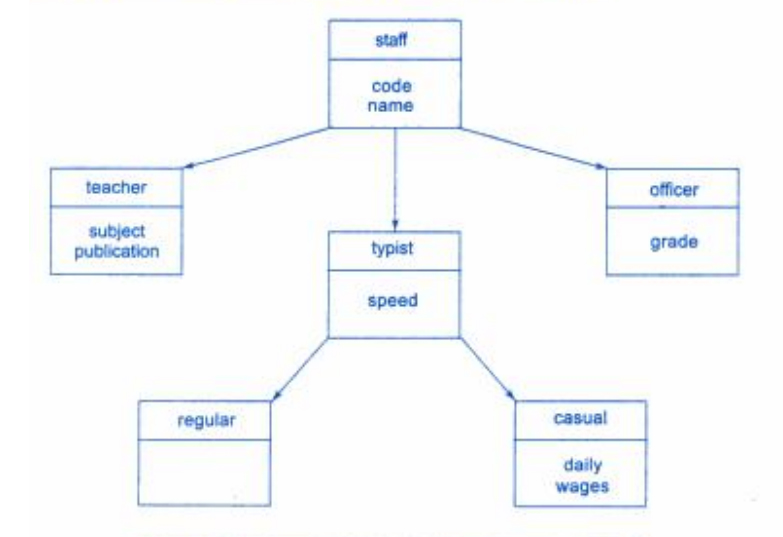
\includegraphics[width=130mm]{cpp_5_3.jpg}
  \label{fig:boat1}
\end{figure}

\end{center}

\textit{Code.}
\begin{lstlisting}
#include<stdio.h>
#include<stdlib.h>
#include<string>
#include<iostream>
using namespace std;
class Staff
{
public:
	string code_name;
	virtual void display()=0;
};
class Teacher : public Staff
{
public:
	string subj;
	string publ;
	void init(string code, string _subj, string _publ)
	{
		code_name=code;
		subj=_subj;
		publ=_publ;
	}
	void display()
	{
		cout<<"Code name: "<<code_name<<endl;
		cout<<"Teacher subj =  "<<subj<<"\tTeacher publ "<<publ;
	}
};
class Typist : public Staff
{
public:
	int speed;
	void init(string code, int s)
	{
		code_name=code;
		speed=s;
	}
	void display()
	{
		cout<<"Code name: "<<code_name<<endl;
		cout<<"Speed of Typist "<<speed;
	}
};
class Officer : public Staff
{
public:
	char grade;
	void init(string code, char g)
	{
		code_name=code;
		grade=g;
	}
	void display()
	{
		cout<<"Code name: "<<code_name<<endl;
		cout<<"Class of Officer "<<grade;
	}
};
class regular : public Typist
{
public:
	void typ(string code, int speed)
	{
		init(code, speed);
	}
	void display()
	{
		cout<<"Code name: "<<code_name<<endl;
		cout<<"Regular Typist\n";
	}
};
class casual : public Typist
{
public:
	int wage;
	void typ(string code, int speed, int _wage)
	{
		init(code, speed);
		wage=_wage;
	}
	void display()
	{
		cout<<"Code name: "<<code_name<<endl;
		cout<<"Daily Wages: "<<wage;
	}
};
int main()
{
	vector<Staff *> database;
	Teacher t;
	t.init("T010", "CSE", "CLRS");
	regular tr;
	tr.typ("TPR010", 2);
	casual cst;
	cst.typ("TRC011",5,500);
	Officer of;
	of.init("OF010", 'C');
	database.push_back(&t);
	database.push_back(&tr);
	database.push_back(&cst);
	database.push_back(&of);
	int i;
	for(i=0;i<database.size();i++) {
		Staff *s=database[i];
		s->display();
	}
	return 0;
}
\end{lstlisting}


\textit{Output.}
\begin{lstlisting}
Code name: T010
Teacher subj =  CSE     Teacher publ CLRSCode name: TPR010
Regular Typist
Code name: TRC011
Daily Wages: 500Code name: OF010
Class of Officer C
\end{lstlisting}


\section{Inheritance - Class Network}
\textbf{Problem 5.4} \textit{Consider a class network as shown below. Define all four classes and write a program to create, update and display the information
contained in master objects.}

\begin{center}


\begin{figure}[h!]
  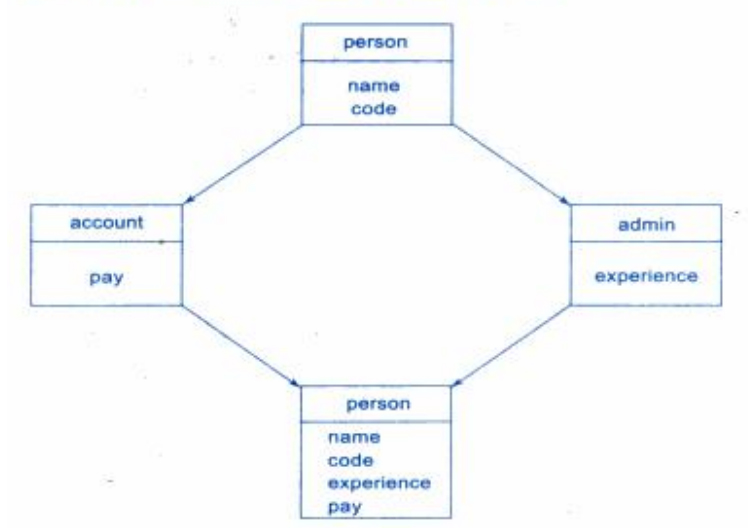
\includegraphics[width=130mm]{cpp_5_4.jpg}
  \label{fig:boat1}
\end{figure}

\end{center}

\textit{Code.}
\begin{lstlisting}
#include<stdio.h>
#include<stdlib.h>
#include<string>
using namespace std;

class master
{
public:
	string name;
	string code;
	//virtual void display()=0;
	void inp(string _name, string _code)
	{
		name=_name;
		code=_code;
	}
};

class account : public master
{
public:
	int pay;
	void init1(string _name, string _code, int _pay)
	{
		inp(_name, _code);
		pay=_pay;
	}
	void display1()
	{
		cout<<"Name: "<<name<<" code: "<<code<<" pay: "<<pay<<endl;
	}
};

class admin : public master
{
public:
	int exp;
	void init2(string _name, string _code, int _exp)
	{
		inp(_name, _code);
		exp=_exp;
	}
	void display2()
	{
		cout<<"Name: "<<name<<" code: "<<code<<" exp: "<<exp<<endl;
	}
};

class person : public admin, public account
{
public:
	void initialise(string _name, string _code, int _exp, int _pay)
	{
		init1(_name, _code, _pay);
		init2(_name, _code, _exp);
	}
	void display()
	{
		display1();
		display2();
	}
};

int main()
{
	person p1;
	p1.initialise("Rudra", "CS101", 2, 0);
	p1.display();
	return 0;
}
\end{lstlisting}


\textit{Output.}
\begin{lstlisting}
Name: Rudra code: CS101 pay: 0
Name: Rudra code: CS101 exp: 2
\end{lstlisting}

\section{Inheritance - Virtual methods}
\textbf{Problem 6.1} \textit{Write a program implementing \textbf{Shape} class, from which Triangle and Rectangle inherit. Use ’virtual’.}

\begin{center}


\end{center}

\textit{Code.}
\begin{lstlisting}
#include<stdio.h>
#include<stdlib.h>
#include<string>
#include<iostream>
#define DEBUG(x) cout<< '>' << #x<<':'<<x<<endl;
using namespace std;
class Shape
{
public:
	double l,b;
	
	void getData(double _l, double _b)
	{
		l=_l;
		b=_b;
	}
	
	virtual void display_area()
	{}
};

class triangle : public Shape
{
	void getData(double _l, double _b)
	{
		l=_l;
		b=_b;
	}
	void display_area()
	{
		double areaTriangle=0.5*l*b;
		DEBUG(areaTriangle)
	}
};
class rectangle : public Shape
{
	void getData(double _l, double _b)
	{
		l=_l;
		b=_b;
	}
	void display_area()
	{
		double areaRectangle=l*b;
		DEBUG(areaRectangle)
	}
};
int main()
{
	Shape *s;
	char ch; // choice
	cout<<"Rectangle(r) or Triangle(t) ? \n";
	cin>>ch;
	if(ch=='r' || ch=='R') {
		rectangle r;
		s=&r;
		double x,y;
		cout<<"Enter the  value of sides\n";
		cin>>x>>y;
		s->getData(x,y);
		s->display_area();
	} else if(ch=='t' || ch=='T') {
		triangle t;
		s=&t;
		double x,y;
		cout<<"Enter the  value of sides\n";
		cin>>x>>y;
		s->getData(x,y);
		s->display_area();
	} else {
		cout<<"Wrong choice";
	}
	return 0;
}
\end{lstlisting}


\textit{Output.}
\begin{lstlisting}
Rectangle(r) or Triangle(t) ? 
r
Enter the  value of sides
45
56
>areaRectangle:2520
\end{lstlisting}

\section{Inheritance - Area of circle}
\textbf{Problem 6.2} \textit{Extend the above program to calculate the area of Circle.}

\textit{Code.}
\begin{lstlisting}
#include<stdio.h>
#include<stdlib.h>
#include<string>
#include<iostream>

#define DEBUG(x) cout<< '>' << #x<<':'<<x<<endl;
#define PI 3.14156

using namespace std;

class Shape
{
public:
	double l,b;
	
	void getData(double _l, double _b)
	{
		l=_l;
		b=_b;
	}
	
	virtual void display_area()
	{}
};

class triangle : public Shape
{
	void getData(double _l, double _b)
	{
		l=_l;
		b=_b;
	}
	void display_area()
	{
		double areaTriangle=0.5*l*b;
		DEBUG(areaTriangle)
	}
};

class rectangle : public Shape
{
	void getData(double _l, double _b)
	{
		l=_l;
		b=_b;
	}
	void display_area()
	{
		double areaRectangle=l*b;
		DEBUG(areaRectangle)
	}
};

class circle : public Shape
{
	void getData(double _l, double _b)
	{
		l=_l;
		b=0;
	}
	void display_area()
	{
		double areaCircle=PI*l*l;
		DEBUG(areaCircle)
	}
};

int main()
{
	Shape *s;
	char ch; // choice
	cout<<"Rectangle(r) or Triangle(t) or Circle (c)? \n";
	cin>>ch;
	if(ch=='r' || ch=='R') {
		rectangle r;
		s=&r;
		double x,y;
		cout<<"Enter the  value of sides\n";
		cin>>x>>y;
		s->getData(x,y);
		s->display_area();
	} else if(ch=='t' || ch=='T') {
		triangle t;
		s=&t;
		double x,y;
		cout<<"Enter the  value of sides\n";
		cin>>x>>y;
		s->getData(x,y);
		s->display_area();
	} else if(ch=='c' || ch=='C') {
		circle c;
		s=&c;
		double x;
		cin>>x;
		s->getData(x,0);
		s->display_area();
	} else {
		cout<<"Wrong choice";
	}
	return 0;
}
\end{lstlisting}


\textit{Output.}
\begin{lstlisting}
Rectangle(r) or Triangle(t) or Circle (c)? 
c
5
>areaCircle:78.539
\end{lstlisting}

\section{Inheritance - Non virtual methods}
\textbf{Problem 6.3} \textit{Modify the above program by removing the virtual keywords from the methods. Comment the result}

\textbf{Result.} \textit{No Change}

\section{Function Template}
\textbf{Problem 7.1} \textit{.Write a Function Template for finding the minimum value contained in an array.}

\textit{Code.}
\begin{lstlisting}
#include <iostream>
using namespace std;

template <typename T>
void find_min(T* a, int n)
{
    T mn=a[0];
    int i;
    for(i=1;i<n;i++) {
        if(mn>a[i]) {
            mn=a[i];
        }
    }
    cout<<"Min is: "<<mn;
}

int main() {
	int n,i;
	cin>>n;
	int a[n];
	float b[n];
	cout<<"Enter int values: "<<endl;
	for(i=0;i<n;i++) {
	    cin>>a[i];
	}
	find_min(a, n);
	cout<<"\nEnter float values: "<<endl;
	for(i=0;i<n;i++) {
	    cin>>b[i];
	}
	find_min(b, n);
	return 0;
}
\end{lstlisting}

\textit{Output.}
\begin{lstlisting}
5
Enter int values: 
5 -1 2 3 4
Min is: -1
Enter float values: 
-2.0 -1.2 5 6 8
Min is: -2
\end{lstlisting}

\section{Vector Operations}
\textbf{Problem 7.2} \textit{.Write a Class Template to represent a generic vector. Include member functions to perform the following tasks. \\
a) To create a vector\\
b) To modify the value of a given vector.\\ 
c) To multiply by a scalar. \\
d) To display the vector in the form of (10,20,30 . . . )}

\textit{Code.}
\begin{lstlisting}
#include<iostream>
#include<vector>

using namespace std;

template <class T>
class vec {
    vector<T> g;
public:
    vec() {}
    void create()
    {
        createUtil();
    }
    void modify()
    {
        T mod, with;
        cout<<"Enter value of element to modify: ";
        cin>>mod;
        cout<<"Enter value to modify to: ";
        cin>>with;
        modifyUtil(mod, with);
    }
    void mult()
    {
        int m;
        cout<<"Enter value to multiply with (int): ";
        cin>>m;
        multUtil(m);
    }
    void display()
    {
        displayUtil();
    }
private:
    void createUtil()
    {
        //cout<<"Press -1 to stop pushing to vector\n";
        T element;
        char ch;
        while(true) {
            cout<<"Want to exit ? [y/n]: ";
            cin>>ch;
            if(ch=='Y'||ch=='y') {
                break;
            }
            cin>>element;
            g.push_back(element);
        }
    }
    void modifyUtil(T mod, T with)
    {
        int i;
        for(i=0;i<g.size();i++) {
            if(g[i]==mod) {
                g[i]=with;
            }
        }
    }
    void multUtil(int m)
    {
        int i;
        for(i=0;i<g.size();i++) {
            g[i]*=m;
        }
    }
    void displayUtil()
    {
        cout<<"Current Vector: \n";
        int i;
        for(i=0;i<g.size();i++) {
            cout<<g[i]<<" "<<endl;
        }
        cout<<"\n---------------------\n";
    }
};

int main()
{
    vec<int> st;
    st.create();
    st.display();
    st.modify();
    st.display();
    st.mult();
    st.display();
    return 0;
}
\end{lstlisting}

\textit{Output.}
\begin{lstlisting}
Want to exit ? [y/n]: n
56
Want to exit ? [y/n]: n
45
Want to exit ? [y/n]: y
Current Vector: 
56 
45 

---------------------
Enter value of element to modify: 56
Enter value to modify to: 89
Current Vector: 
89 
45 

---------------------
Enter value to multiply with (int): 2
Current Vector: 
178 
90 

---------------------
\end{lstlisting}

\section{Multi catch statements}
\textbf{Problem 8.1} \textit{Write a program that illustrates multi-catch statements}

\textit{Code.}
\begin{lstlisting}
#include<iostream>
using namespace std;
void exep(int a, int b)
{
	if(a==b) {
		throw 0;
	} else {
		throw 1.0f;
	}
}
void check(int a, int b)
{
	try {
		exep(a,b);
	} catch (int x) {
		cout<<"Equal no.s\n";
	} catch (float x) {
		cout<<"Unequal no.s\n";
	}
}
int main()
{
	check(10,10);
	check(10,20);
}
\end{lstlisting}

\textit{Code.}
\begin{lstlisting}
Equal no.s
Unequal no.s
\end{lstlisting}

\section{Re-throwing exceptions}
\textbf{Problem 8.2} \textit{Write a program that illustrates rethrowing of exceptions}

\textit{Code.}
\begin{lstlisting}
#include<iostream>
using namespace std;
void exep()
{
	int x=1,y=2;
	if((y-x)==2)
		throw 'A';
	else
		throw 'B';
}
int main()
{
	try {
		exep();
	} catch(char ch) {
		if(ch=='A') {
			cout<<"Done\n";
		} else {
			throw 0;
		}
	}
}
\end{lstlisting}

\textit{Output.}
\begin{lstlisting}
terminate called after throwing an instance of 'int'
[1]    7083 abort (core dumped)  ./a.out
\end{lstlisting}

\end{document}
\grid
